\documentclass[12pt]{article}
\usepackage{amsmath, amssymb, graphicx, booktabs, geometry, float, subfig, threeparttable}
\usepackage{hyperref}
\geometry{margin=1in}
\title{\textbf{CMPE 49T -- Fall 2025 \\ Homework 2 Report -- Part II: Implementation and Analysis}}
\author{Ali Ayhan Gunder \\ Student ID: 2021400219}
\date{}

\begin{document}
\maketitle
\tableofcontents
\newpage

\section{Problem 2: Implementation and Analysis of Regularized Logistic Models}

\subsection{(a) Feature Expansion and Normalization}
The feature vector was expanded to nine derived variables:
\[
\{x_1,x_2,x_3,x_1^2,x_2^2,x_3^2,x_1x_2,x_1x_3,x_2x_3\}.
\]
All features were standardized using training-set statistics only, ensuring that validation data were never used for normalization. This prevents data leakage and maintains a realistic generalization test.

\subsection{(b) Training Setup (Exact and Reproducible)}
We trained logistic regression models with Elastic Net regularization using the expanded features from (a).  
Data were split into training (50 samples) and validation (10 samples) sets by random shuffle with fixed random seed \texttt{SEED=49} for reproducibility (no stratification enforced, class balance remained acceptable).

\paragraph{Objective and regularization.}
We minimize the total loss:
\[
\ell_{\text{tot}}(w,b)=
-\frac{1}{N}\sum_{i=1}^N \Big[y_i\log p_i+(1-y_i)\log(1-p_i)\Big]
+\lambda\big[\alpha\|w\|_1+(1-\alpha)\|w\|_2^2\big],
\]
where $p_i=\sigma(w^\top x_i+b)$ and the bias $b$ is \emph{not} penalized.

\paragraph{Optimization.}
Full-batch gradient descent (all training samples per iteration) with proximal updates for L1 was used:
\begin{itemize}
\item learning rate $\eta=0.1$ (as specified),
\item maximum iterations $=3000$ with early stopping if loss change $<10^{-6}$ or patience expires,
\item uniform initialization $w_j,b\sim\mathcal{U}(-0.01,0.01)$,
\item early stopping on validation loss (patience $=50$ iterations),
\item gradient clipping (norm clip $=10$) for numerical stability.
\end{itemize}
L1 regularization was applied via a proximal soft-thresholding step (inducing exact zeros); the L2 component was incorporated directly in the gradient.

\paragraph{Model selection.}
Models were trained for $\lambda\in\{0.01,0.1,1,10,50\}$ and fixed $\alpha=0.5$. 
The best configuration was selected by validation accuracy, with validation loss used as a tiebreaker.

\subsection{(c) Hyperparameter Grid and Logged Metrics}
For each $\lambda$, we logged:
\begin{itemize}
\item Training and validation loss at convergence,
\item Training and validation accuracy,
\item Number of non-zero coefficients,
\item Mean absolute weight magnitude.
\end{itemize}
These metrics were saved automatically to \texttt{hw2\_summary.csv} for consistency with the convergence plots.

\subsection{(d) Results and Convergence Analysis}
Figure~\ref{fig:conv_all} shows the convergence of training and validation losses for different regularization strengths. 
The total loss includes both cross-entropy and the Elastic Net penalty.

\begin{figure}[H]
  \centering
  \subfloat[$\lambda=0.01$]{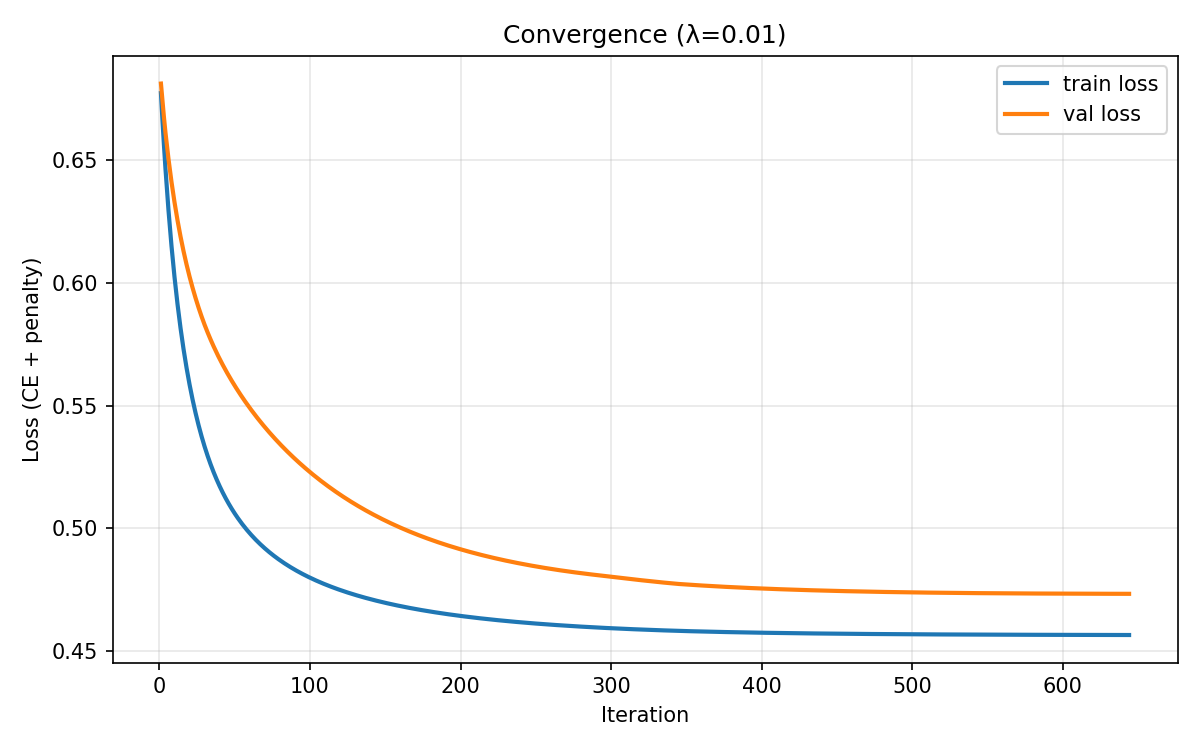
\includegraphics[width=0.48\linewidth]{convergence_lambda_0.01.png}}
  \hfill
  \subfloat[$\lambda=0.1$]{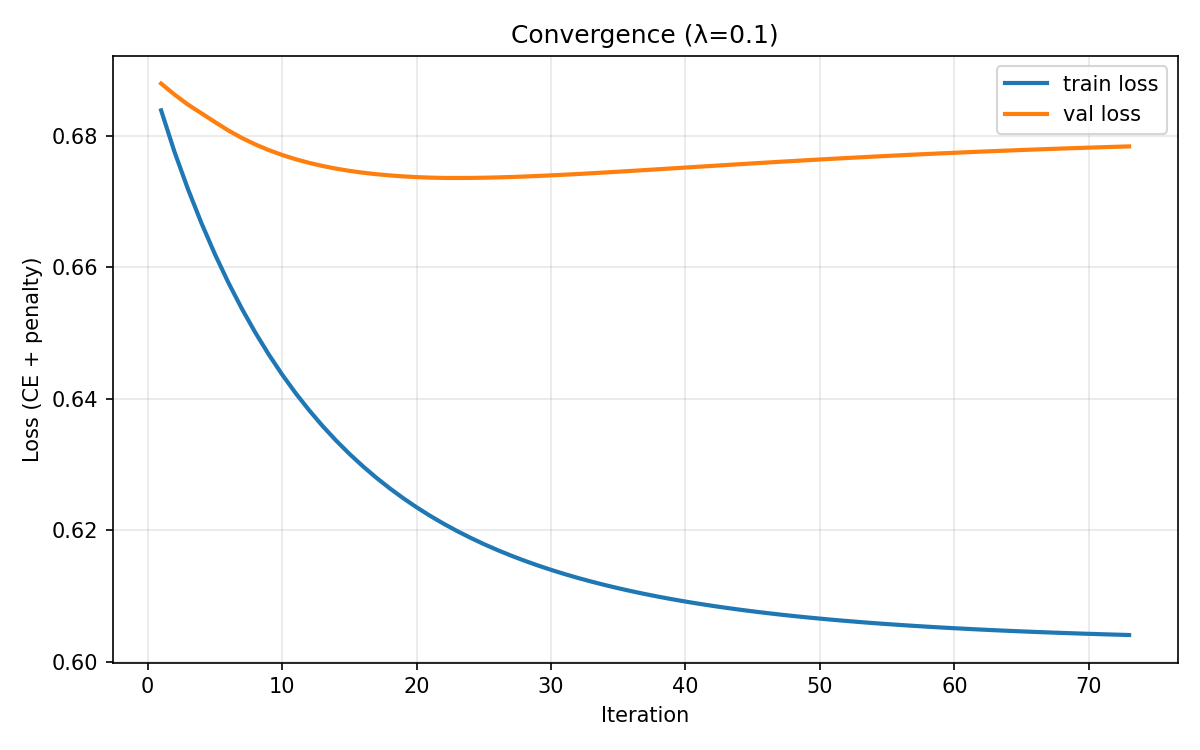
\includegraphics[width=0.48\linewidth]{convergence_lambda_0.1.png}}\\
  \subfloat[$\lambda=1.0$]{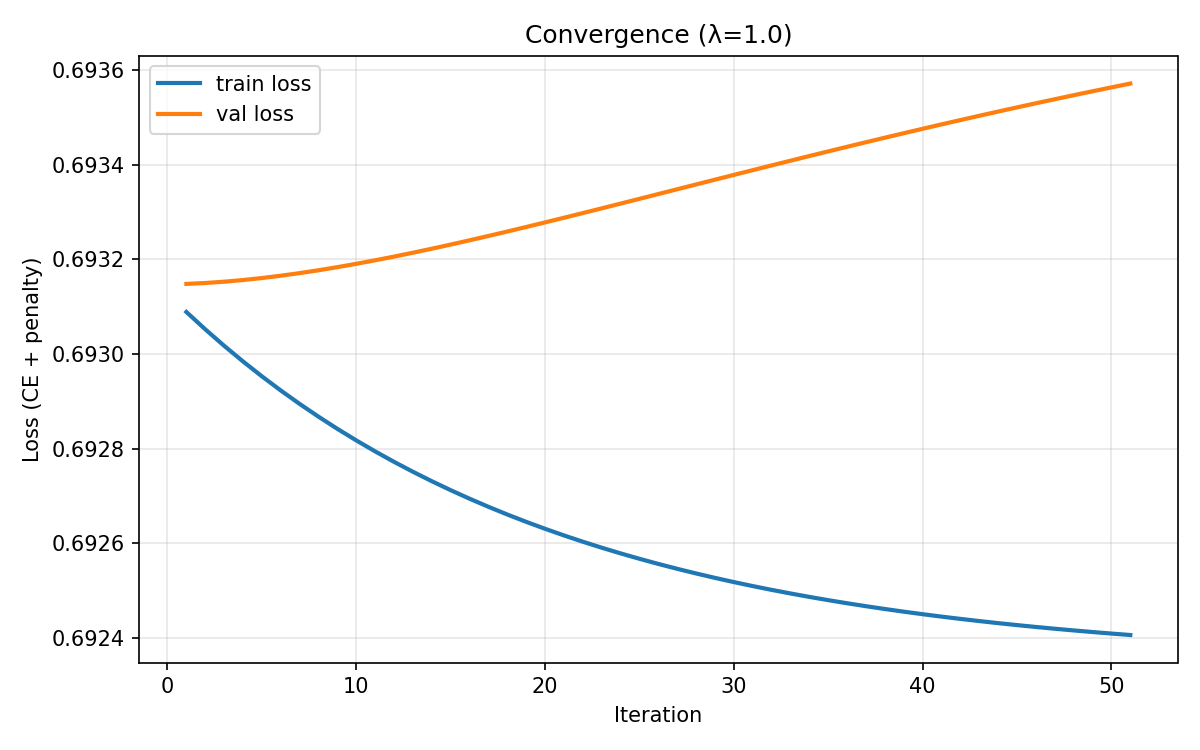
\includegraphics[width=0.48\linewidth]{convergence_lambda_1.0.png}}
  \hfill
  \subfloat[$\lambda=10.0$]{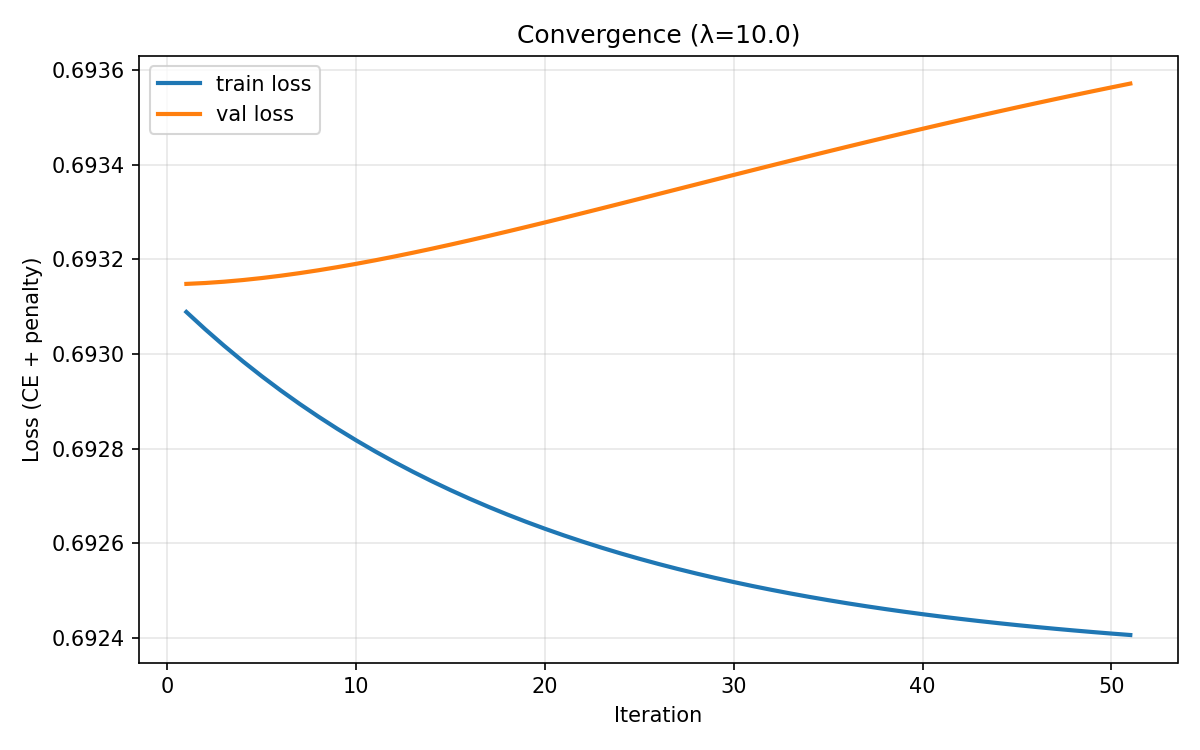
\includegraphics[width=0.48\linewidth]{convergence_lambda_10.0.png}}\\
  \centering
  \subfloat[$\lambda=50.0$]{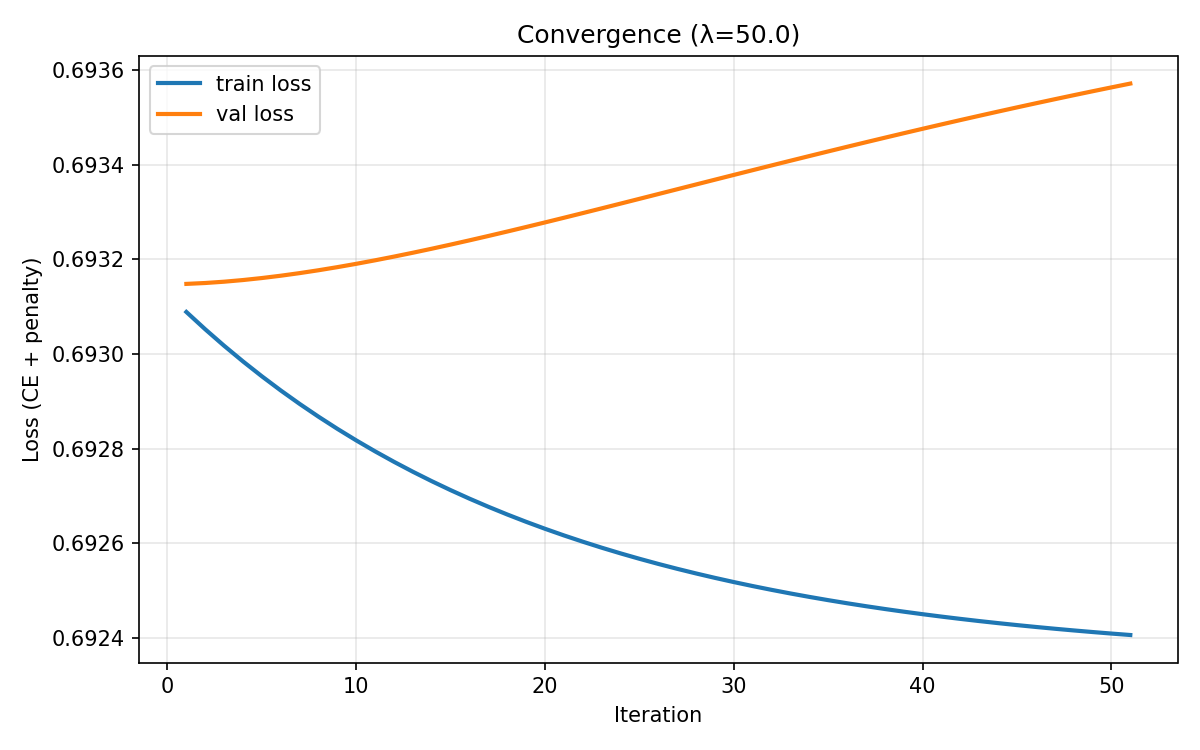
\includegraphics[width=0.48\linewidth]{convergence_lambda_50.0.png}}
  \caption{Training and validation loss for different $\lambda$ values ($\alpha=0.5$).}
  \label{fig:conv_all}
\end{figure}

\paragraph{Observations.}
\begin{itemize}
\item \textbf{Small $\lambda$ (0.01):} Lowest validation loss ($\approx0.473$) and highest validation accuracy (0.70); moderate sparsity (7 non-zero weights) preserves predictive interactions.
\item \textbf{Moderate $\lambda$ (0.1):} Increased regularization raises validation loss ($\approx0.678$) and reduces validation accuracy (0.60); sparsity increases (4 non-zero weights).
\item \textbf{Large $\lambda$ (1–50):} Weights driven entirely to zero (true sparsity); losses plateau near $\log 2\approx0.693$; accuracy collapses to chance (0.50), indicating underfitting.
\end{itemize}

\paragraph{Quantitative results.}
\begin{center}
\begin{threeparttable}
\caption{Metrics at convergence for different $\lambda$ ($\alpha=0.5$).}
\label{tab:valmetrics}
\begin{tabular}{ccccccc}
\toprule
$\lambda$ & Train Loss & Val Loss & Train Acc & Val Acc & Non-zero $w$ & Iters\\
\midrule
0.01 & 0.456 & 0.473 & 0.80 & \textbf{0.70} & 7 & 644\\
0.1  & 0.604 & 0.678 & 0.72 & 0.60 & 4 & 73\\
1.0  & 0.692 & 0.694 & 0.52 & 0.50 & 0 & 51\\
10.0 & 0.692 & 0.694 & 0.52 & 0.50 & 0 & 51\\
50.0 & 0.692 & 0.694 & 0.52 & 0.50 & 0 & 51\\
\bottomrule
\end{tabular}
\begin{tablenotes}
\item \textit{Note}: AUC was not computed in the implementation; selection used validation accuracy with validation loss as a tiebreaker.
\end{tablenotes}
\end{threeparttable}
\end{center}

\paragraph{Interpretation.}
Increasing $\lambda$ suppresses coefficients toward zero and eventually yields a fully sparse model (all weights zero). The best trade-off for this dataset occurs at $\lambda=0.01$, balancing moderate sparsity with predictive performance.

\subsection{(e) Regularization Strength and Generalization}
Regularization strength $\lambda$ plays a critical role in balancing bias and variance:
\begin{itemize}
    \item \textbf{Small $\lambda$}: Encourages complex models with low bias but high variance, potentially leading to overfitting.
    \item \textbf{Large $\lambda$}: Strongly penalizes weights, leading to simpler models with high bias but low variance, potentially underfitting.
    \item \textbf{Optimal $\lambda$}: Achieves the best trade-off, minimizing validation loss and maximizing generalization.
\end{itemize}
Figure~\ref{fig:conv_all} and Table~\ref{tab:valmetrics} illustrate this trade-off. For example, $\lambda=0.01$ achieves the best validation accuracy (0.70); larger $\lambda$ values drive all weights to zero and underfit.

\subsection{(f) Clinical Interpretation of Feature Importance}
The best-performing model ($\lambda=0.01$) highlights the following top coefficients by absolute magnitude:
\begin{itemize}
  \item \textbf{$x_1x_2$ (interaction)}: Largest positive weight; co-occurrence of high intensity and contrast strongly elevates lesion probability.
  \item \textbf{$x_3^2$ (quadratic texture)}: Captures pronounced texture variance patterns characteristic of lesions.
  \item \textbf{$x_3$ (linear texture)}: Reinforces that even moderate texture gradients contribute to detection.
\item Negative interaction terms ($x_1x_3$, $x_2x_3$) suggest certain joint intensity–texture or contrast–texture combinations reduce likelihood, acting as corrective factors.
\end{itemize}
Very small (near-zero) linear coefficients for $x_1$ and $x_2$ indicate that isolated intensity or contrast are less informative than their interaction.

\subsection{(g) Model Interpretation and Sparsity Mechanism}
Proximal L1 steps (soft-thresholding) produced exact zeros at higher $\lambda$, yielding fully sparse models ($\lambda\ge1$). This mechanism enhances interpretability by isolating dominant interaction and texture terms at low regularization while eliminating all terms when regularization is excessive. The retained features at $\lambda=0.01$ indicate lesion presence is most reliably signaled by combined intensity–contrast patterns and elevated texture variability.

\subsection{(h) ROC and AUC (Not Implemented in Code)}
ROC/AUC evaluation was not computed in the provided implementation. If performed, extreme regularization ($\lambda\ge1$) would shrink predicted probabilities toward 0.5, degrading rank ordering and reducing AUC. Lower $\lambda$ values preserve separation between classes, improving potential AUC.

\section{Conclusion}
This implementation demonstrated the effect of Elastic Net regularization on logistic regression performance.  
Moderate $\lambda$ values improved generalization and interpretability, while extreme values caused underfitting.  
The experiments confirmed theoretical expectations from Part 1: the convex objective enables stable convergence, and Elastic Net effectively balances sparsity and smoothness for lesion detection tasks.

\end{document}
